%%%%%%%%%%%%%%%%%%%%%%%%%%%%%%%%%%%%%%%%%%%%%%%%%%%%%%%%%%%%%%%%%%%%%%%%%%%%%%%%
%Tutorial slides on Python.
%
% Author: FOSSEE
% Copyright (c) 2009-2016, FOSSEE, IIT Bombay
%%%%%%%%%%%%%%%%%%%%%%%%%%%%%%%%%%%%%%%%%%%%%%%%%%%%%%%%%%%%%%%%%%%%%%%%%%%%%%%%

\documentclass[14pt,compress]{beamer}

% Modified from: generic-ornate-15min-45min.de.tex
\mode<presentation>
{
  \usetheme{Warsaw}
  \useoutertheme{infolines}
  \setbeamercovered{transparent}
}

% Remove navigation symbols.
\setbeamertemplate{navigation symbols}{}

\usepackage[english]{babel}
\usepackage[latin1]{inputenc}
%\usepackage{times}
\usepackage[T1]{fontenc}

% Taken from Fernando's slides.
\usepackage{ae,aecompl}
\usepackage{mathpazo,courier,euler}
\usepackage[scaled=.95]{helvet}

\definecolor{darkgreen}{rgb}{0,0.5,0}

\usepackage{listings}
\lstset{language=Python,
    basicstyle=\ttfamily\bfseries,
    commentstyle=\color{red}\itshape,
  stringstyle=\color{darkgreen},
  showstringspaces=false,
  keywordstyle=\color{blue}\bfseries}

%%%%%%%%%%%%%%%%%%%%%%%%%%%%%%%%%%%%%%%%%%%%%%%%%%%%%%%%%%%%%%%%%%%%%%
% Macros
\setbeamercolor{emphbar}{bg=blue!20, fg=black}
\newcommand{\emphbar}[1]
{\begin{beamercolorbox}[rounded=true]{emphbar}
      {#1}
 \end{beamercolorbox}
}
\newcounter{time}
\setcounter{time}{0}
\newcommand{\inctime}[1]{\addtocounter{time}{#1}{\tiny \thetime\ m}}

\newcommand{\typ}[1]{\lstinline{#1}}

\newcommand{\kwrd}[1]{ \texttt{\textbf{\color{blue}{#1}}}  }

\newcommand\BackgroundPicture[1]{%
  \setbeamertemplate{background}{%
      \parbox[c][\paperheight]{\paperwidth}{%
      \vfill \hfill
        \pgfimage[width=1.0\paperwidth,height=1.0\paperheight]{#1}
 \hfill \vfill
}}}

% For non-wide pictures, set the width so that the height scales
% appropriately.
\newcommand\BackgroundPictureWidth[1]{%
  \setbeamertemplate{background}{%
      \parbox[c][\paperheight]{\paperwidth}{%
      \vfill \hfill
        \pgfimage[width=1.0\paperwidth]{#1}
 \hfill \vfill
}}}

% For shorter pictures, set the height so that the width scales
% appropriately.
\newcommand\BackgroundPictureHeight[1]{%
  \setbeamertemplate{background}{%
      \parbox[c][\paperheight]{\paperwidth}{%
      \vfill \hfill
        \pgfimage[height=1.0\paperheight]{#1}
 \hfill \vfill
}}}

%%%%%%%%%%%%%%%%%%%%%%%%%%%%%%%%%%%%%%%%%%%%%%%%%%%%%%%%%%%%%%%%%%%%%%
% Title page
\title[Preliminaries]{Introductory Scientific Computing with
Python}
\subtitle{Some preliminaries}

\author[FOSSEE] {FOSSEE}

\institute[IIT Bombay] {Department of Aerospace Engineering\\IIT Bombay}
\date[] {Mumbai, India
}
%%%%%%%%%%%%%%%%%%%%%%%%%%%%%%%%%%%%%%%%%%%%%%%%%%%%%%%%%%%%%%%%%%%%%%

%\pgfdeclareimage[height=0.75cm]{iitmlogo}{iitmlogo}
%\logo{\pgfuseimage{iitmlogo}}


%% Delete this, if you do not want the table of contents to pop up at
%% the beginning of each subsection:
\AtBeginSubsection[]
{
  \begin{frame}<beamer>
    \frametitle{Outline}
    \tableofcontents[currentsection,currentsubsection]
  \end{frame}
}

\AtBeginSection[]
{
  \begin{frame}<beamer>
    \frametitle{Outline}
    \tableofcontents[currentsection,currentsubsection]
  \end{frame}
}

% If you wish to uncover everything in a step-wise fashion, uncomment
% the following command:
%\beamerdefaultoverlayspecification{<+->}

%%\includeonlyframes{current,current1,current2,current3,current4,current5,current6}

%%%%%%%%%%%%%%%%%%%%%%%%%%%%%%%%%%%%%%%%%%%%%%%%%%%%%%%%%%%%%%%%%%%%%%
% DOCUMENT STARTS
\begin{document}

\begin{frame}
  \maketitle
\end{frame}

\begin{frame}[plain]
  \frametitle{What is Python?}
  \large
  \begin{itemize}
  \item Python: the programming language

    \vspace*{0.5in}
  \item \typ{python}: the interpreter
  \end{itemize}
\end{frame}

\begin{frame}[fragile]
  \frametitle{The interpreter}
  \small
  \begin{lstlisting}
$ python
Python 2.7.9 (default, Feb 10 2015, 03:29:10)
Type "help", "copyright", "credits" or "license" for more information.
>>>
\end{lstlisting} %$
\end{frame}

\begin{frame}[fragile]
  \frametitle{The interpreter}
  \small
\begin{lstlisting}
$ python hello.py
hello world
$
\end{lstlisting}
\end{frame}

\begin{frame}[plain]
  \frametitle{Python standard library}
  \begin{itemize}
  \item Built-in
  \item ``Batteries included''
  \item Lot of important functionality
  \end{itemize}
\end{frame}

\begin{frame}[plain]
  \frametitle{Python packages}
  \begin{itemize}
  \item Many other packages available
  \item \typ{ipython}
  \item \typ{numpy}
  \item \typ{scipy}
  \item \typ{matplotlib}
  \item \typ{PyQt}
  \item \typ{django}
  \item \typ{mayavi}
  \item About 1 lakh packages!
  \end{itemize}
\end{frame}

\begin{frame}[plain]
  \frametitle{Official Python}
  \begin{center}
    \url{www.python.org/downloads}

    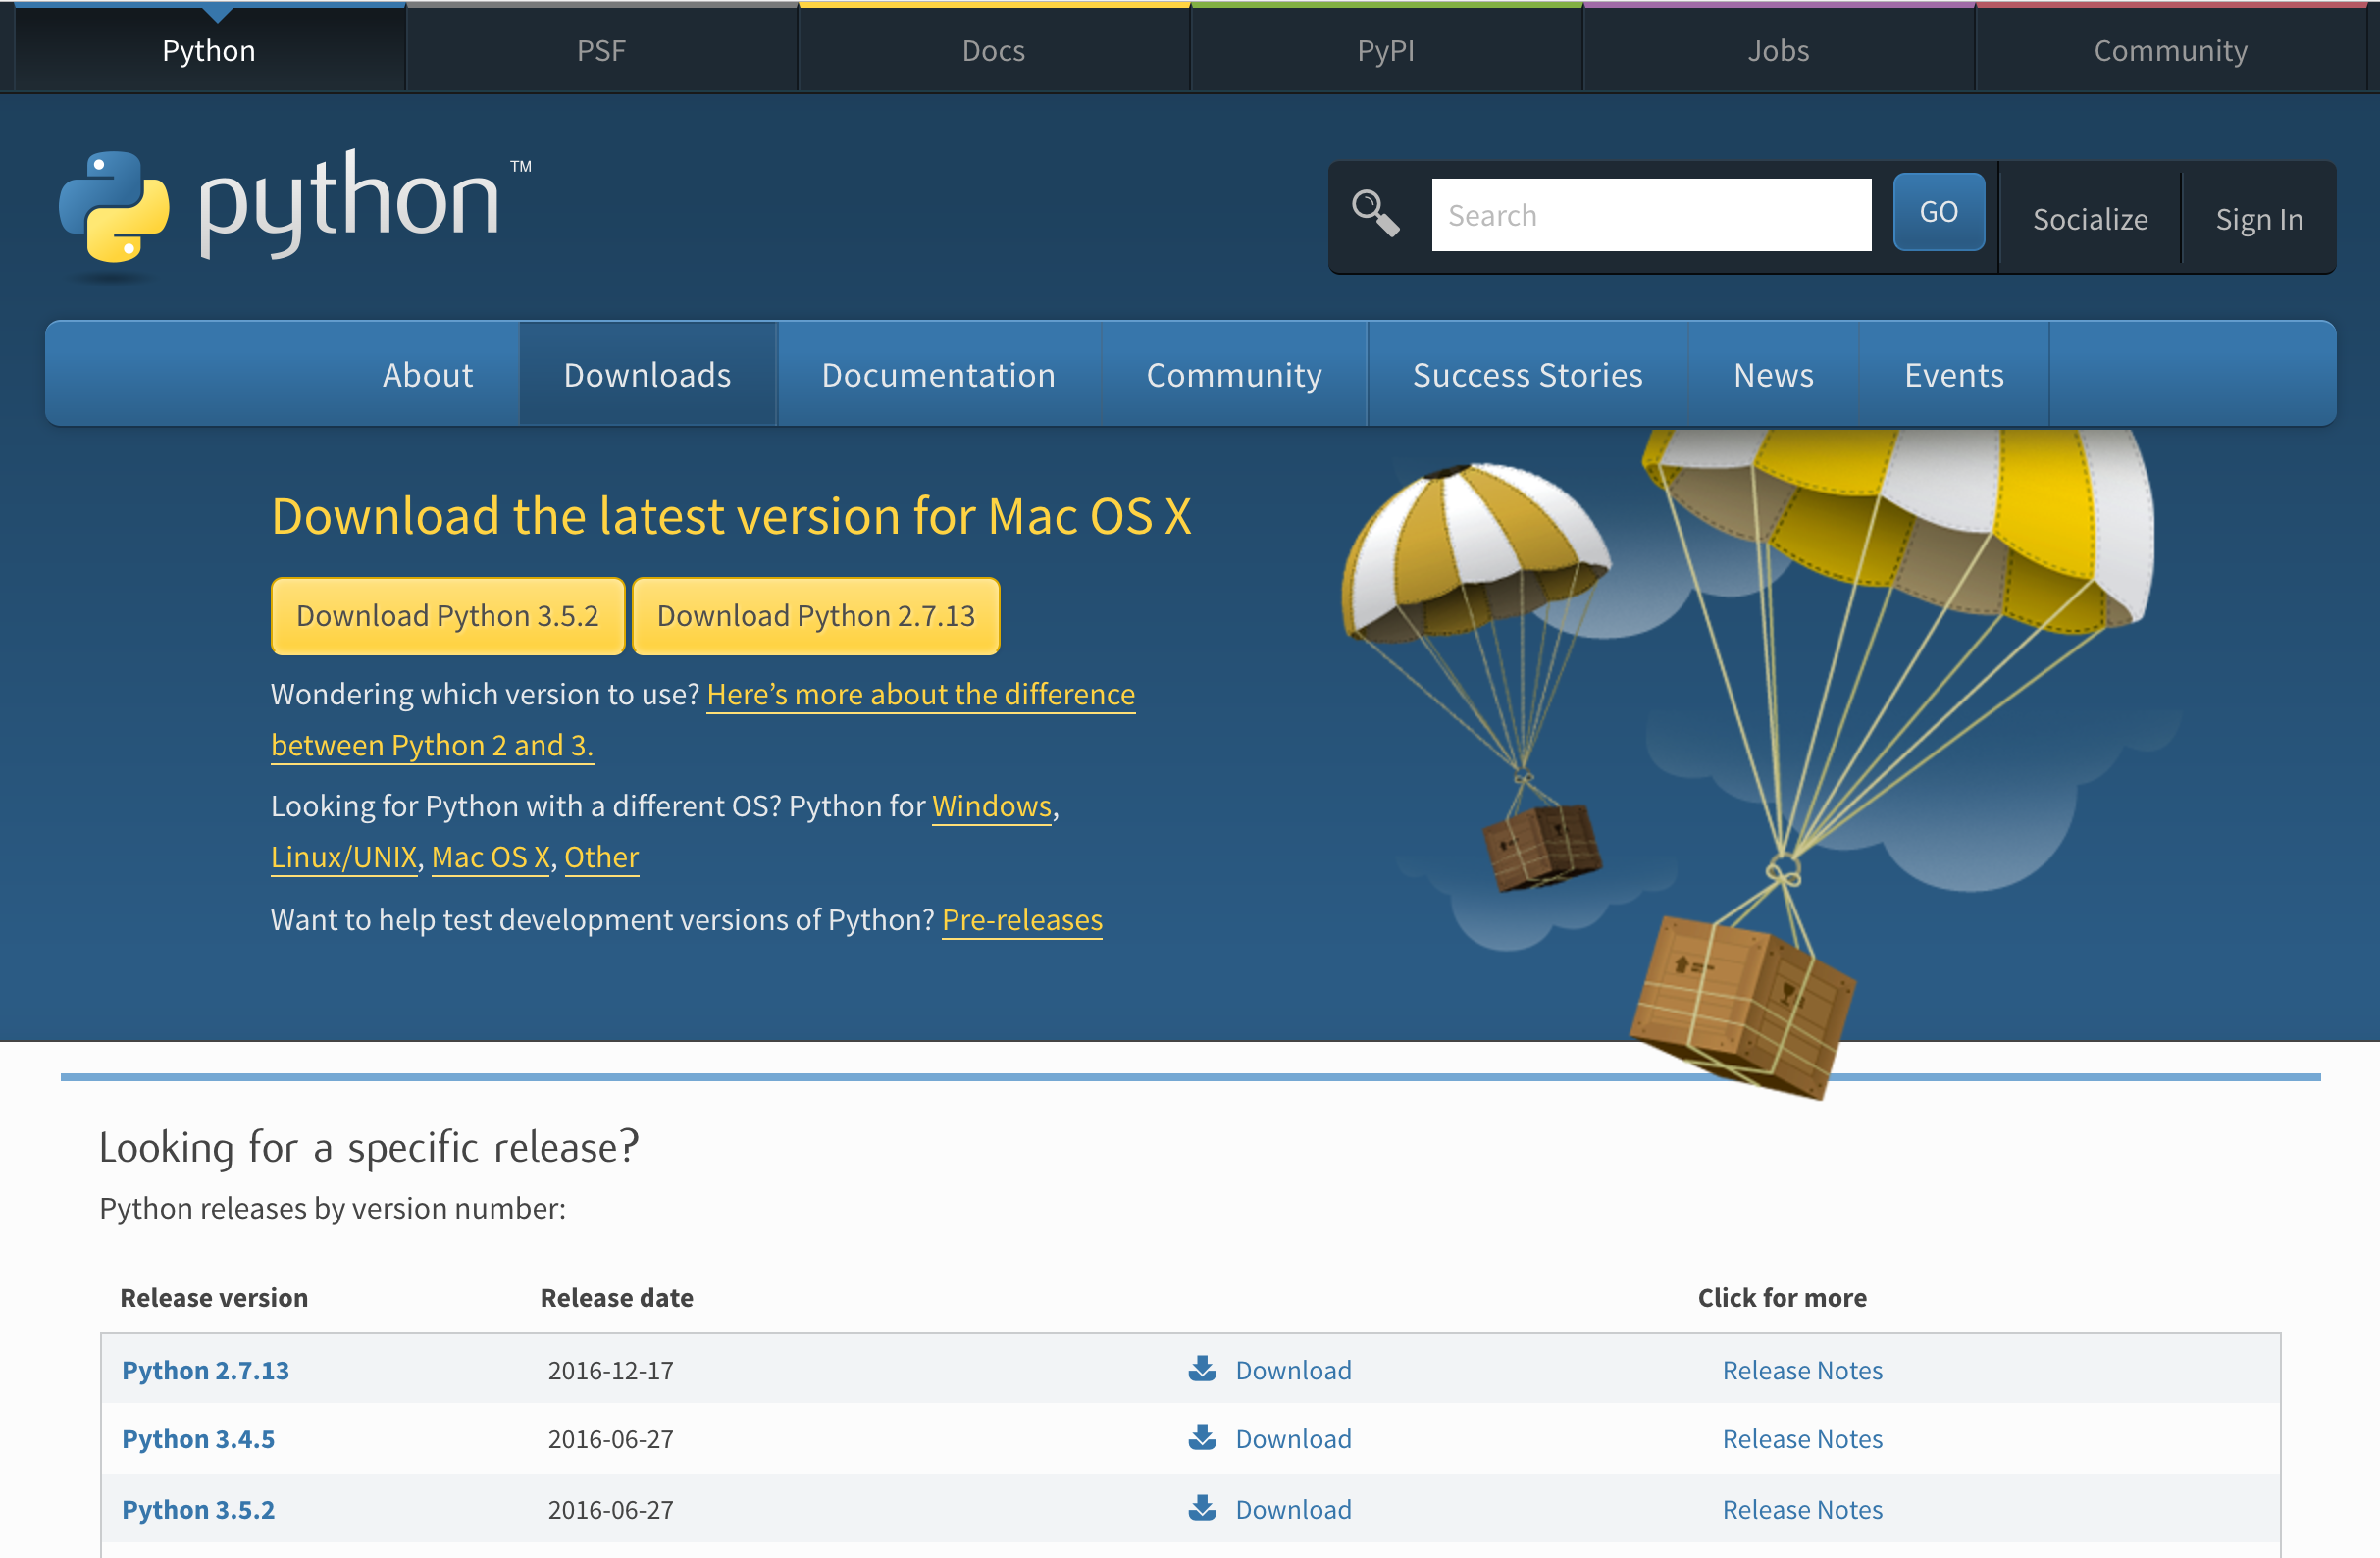
\includegraphics[height=2.75in]{data/intro/python_download}
  \end{center}
\end{frame}

\begin{frame}
  \frametitle{Python distributions}
  \begin{itemize}
  \item GNU/Linux: easy to install
  \item Usually many packages are easy to install
  \item Example: \typ{apt-get}, \typ{yum} etc.
  \item Not so easy on OS X and Windows
  \end{itemize}
\end{frame}

\begin{frame}
  \frametitle{Python distribution: Canopy}
  \begin{itemize}
  \item \url{www.enthought.com/products/canopy}
  \item Easy to use
  \item Simple IDE
  \item Cross platform: Linux, OSX, Windows
  \item Free installer
  \item Many packages
  \end{itemize}
\end{frame}

\begin{frame}
  \frametitle{Python distribution: Anaconda}
  \begin{itemize}
  \item \url{www.continuum.io/downloads}
  \item Cross platform: Linux, OSX, Windows
  \item Free installer
  \item Many packages
  \end{itemize}
\end{frame}

\begin{frame}[plain]
  \frametitle{For this course}
  \begin{itemize}
  \item Using Canopy
  \item Simple UI
  \item Easy for beginners
    \vspace*{0.25in}
  \item Advanced users can use anything they want!
  \end{itemize}
\end{frame}

\begin{frame}[plain]
  \frametitle{Setup}
  \begin{itemize}
    \item Download for your platform
    \item Install it
    \item Start Canopy
  \end{itemize}
\end{frame}

\begin{frame}[plain]
  \frametitle{Summary}
  \begin{itemize}
  \item Python: the programming language
  \item \typ{python}: the interpreter
  \item Python standard library
  \item Other Python packages
  \item Python distributions
  \end{itemize}
\end{frame}




\end{document}
